This subsection shows the avg. of \emph{User Profile 1}'s results, the avg. of \emph{User Profile 2}'s results and the avg. between the two. We have chosen to give you also the separates view of the two groups to better understand how different segments react to the same tasks.

\subsection{Avg. User Profile 1}


\subsection{Avg. User Profile 2}
{
\captionof{table}{Avg per task}
\centering
\begin{tabular}{lllllll} 
	\toprule
	\textbf{Scenario } & \textbf{Task} & \begin{tabular}[c]{@{}l@{}}\textbf{Execution}\\\textbf{Time (s)}\end{tabular} & 			\textbf{Success} & \begin{tabular}[c]{@{}l@{}}\textbf{Perceived}\\\textbf{Difficulty}\end{tabular} & \textbf{Errors} & 			\textbf{Satisfaction}  \\
	Scenario 1 & 1             & 15,25                 	& 100\%          	& 0					& 0					& 5           	                                                                 \\
	Scenario 1 & 2             & 8                   	& 100\%          	& 0					& 0					& 5                                                                                \\
	Scenario 1 & 3             & 19                 	& 100\%          	& 1,5				& 7					& 3,75                                                                               \\
	Scenario 2 & 1             & 10,75                 	& 100\%          	& 0,25				& 1					& 4,75                                                                              \\
	Scenario 2 & 2             & 8,5                   	& 100\%        	& 0					& 0					& 5                                                                                \\
	Scenario 2 & 3             & 9,75                 	& 100\%          	& 1					& 2					& 4                                                                                \\
	Scenario 3 & 1             & 15,25                 	& 100\%         	& 0					& 0					& 5                                                                                \\
	Scenario 3 & 2             & 15                 	& 100\%          	& 0					& 0					& 5                                                                                \\
	Scenario 3 & 3             & 14,5                	& 100\%          	& 0,25				& 0					& 4,5                                                                                 \\
\bottomrule
\end{tabular}

\vspace{1cm}
}It is possibile to see that for this segment the 3 task of scenario 1 has been the most complex and difficult and it can be seen becase the execution time is the heigher as the number of mistakes made and the satisfaction rate is the lower one. \\
The next figure has the aim to show the avg between all scenarios.

\begin{figure}[h!]
	\centering
	\begin{minipage}[b]{1\textwidth}
    		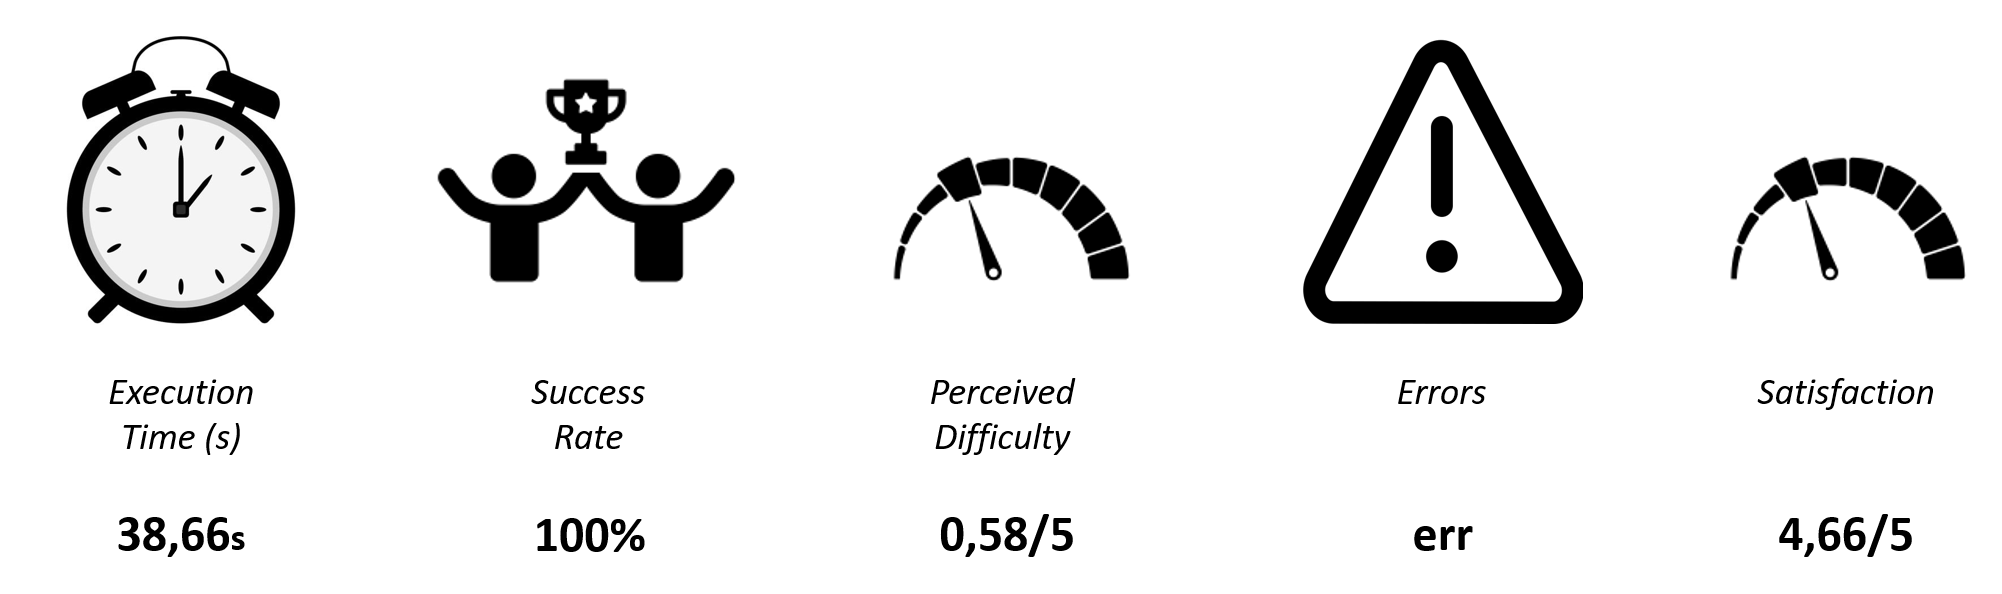
\includegraphics[width=\textwidth]{./assets/avg-2.png}
		\caption{Total Avg. \emph{user profile 2}}
	\end{minipage}
\end{figure}


\subsection{Total Avg.}
